\documentclass[mathserif,serif]{beamer}
\usepackage{tabularx}
\setbeamertemplate{footline}[frame number]
\title{Cut optimization}
\author
{
Samuel Lo \inst{1}
\and
Yanjun Tu  \inst{1}
\and
Dongliang Zhang  \inst{2}
}
\institute
{
\inst{1}
The University of Hong Kong
\and
\inst{2}
University of Michigan
}
\date{\today}

\newcommand\Wider[2][3em]{%
\makebox[\linewidth][c]{%
\begin{minipage}{\dimexpr\textwidth+#1\relax}
\raggedright
\centering#2
\end{minipage}%
}%
}

\begin{document}
\frame{\titlepage}

\begin{frame}
\frametitle{Update}
\begin{itemize}
\normalsize
\item Use 33 fb$^{-1}$ Data
\item No pile up weight is applied
\item Separate the SR into 18*3 bins

\item Get the number of event of signal before normalization
\end{itemize}
\end{frame}

\begin{frame}
\begin{center}
\huge
Signal Region
\end{center}
\end{frame}

\begin{frame}
\frametitle{Signal Region}
Definition of the Signal Region.
\begin{enumerate}
\item Exactly two same sign $ee$, $\mu\mu$ or $e\mu$
\item pt1 $>$ 25 (20) and pt2 $>$ 15 (10) for electron (muon)
\item Events are vetoed if they contain an OSSF pair formed from loose $e$ or $\mu$ in a 15 GeV window around the Z boson mass.(Don't understand the meaning, difficult to implement)
\item Definition of ISR jet: $|\eta| < 2.4$ and $p_T > 40$ GeV
\item The minimum $M_T$ of the two leptons
\end{enumerate}
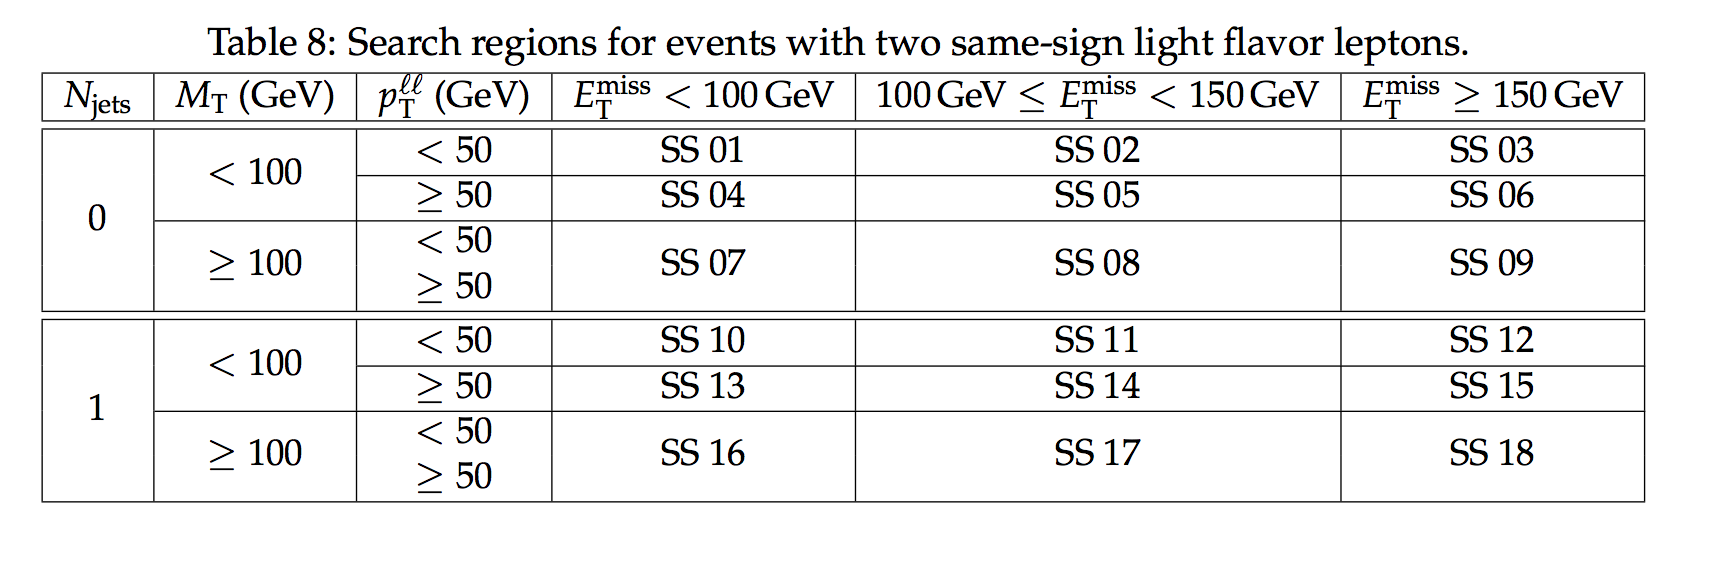
\includegraphics[width=1\textwidth]{data/SR.png}
\end{frame}

\begin{frame}
\frametitle{Result}
\tiny
https://gitlab.cern.ch/hku/SUSY2L/blob/master/code/ \\
plotScripts/dataMCcomparison/latex/data/expN/SR.txt \\
https://docs.google.com/spreadsheets/d/1T7FXh6uskJh4ZMcWxLInByJsAwVqD190krBeaDkWkks/edit
\end{frame}

%\begin{frame}
\frametitle{Expected number of events (For same sign)}
For ee channel, non-ISR\\
\vspace{5mm}
\begin{tabular}{|c|c|c|}
\hline
& Number of events & Significance \\
\hline
VV & $601.3\pm15.5$ & \\
\hline
V$+\gamma$ & $1614.9\pm25.9$ & \\
\hline
charge flip & $33005.0\pm26.4$ & \\
\hline
fake lepton & $2689.9\pm33.3$ & \\
\hline
Total BG & $37911.1\pm52.1$ & \\
\hline
Signal (400, 350) & $9.5\pm1.0$ &$-0.198$\\
\hline
Signal (400, 300) & $12.4\pm1.5$ &$-0.198$\\
\hline
Signal (400, 200) & $9.4\pm1.5$ &$-0.198$\\
\hline

\end{tabular}
\end{frame}

\begin{frame}
\frametitle{Expected number of events (For same sign)}
For $\mu\mu$ channel, non-ISR\\
\vspace{5mm}
\begin{tabular}{|c|c|c|}
\hline
& Number of events & Significance \\
\hline
VV & $625.3\pm5.6$ & \\
\hline
V$+\gamma$ & $4.0\pm0.7$ & \\
\hline
fake lepton & $1180.6\pm8.4$ & \\
\hline
Total BG & $1809.8\pm10.2$ & \\
\hline
Signal (400, 380) & $2.7\pm0.1$ &$-0.194$\\
\hline
Signal (400, 350) & $6.3\pm0.2$ &$-0.187$\\
\hline
Signal (400, 300) & $7.4\pm0.2$ &$-0.185$\\
\hline
Signal (400, 200) & $6.5\pm0.2$ &$-0.187$\\
\hline
Signal (400, 100) & $4.9\pm0.2$ &$-0.190$\\
\hline

\end{tabular}
\end{frame}

\begin{frame}
\frametitle{Expected number of events (For same sign)}
For e$\mu$ channel, non-ISR\\
\vspace{5mm}
\begin{tabular}{|c|c|c|}
\hline
& Number of events & Significance \\
\hline
VV & $1063.0\pm34.3$ & \\
\hline
V$+\gamma$ & $556.8\pm20.4$ & \\
\hline
charge flip & $89.5\pm0.5$ & \\
\hline
fake lepton & $6894.1\pm46.1$ & \\
\hline
Total BG & $8603.4\pm60.9$ & \\
\hline
Signal (400, 380) & $6.6\pm0.3$ &$-0.196$\\
\hline
Signal (400, 350) & $29.9\pm0.7$ &$-0.187$\\
\hline
Signal (400, 300) & $36.9\pm1.0$ &$-0.185$\\
\hline
Signal (400, 200) & $28.0\pm1.0$ &$-0.188$\\
\hline
Signal (400, 100) & $24.6\pm1.2$ &$-0.189$\\
\hline

\end{tabular}
\end{frame}

\begin{frame}
\frametitle{Expected number of events (For same sign)}
For ee channel, ISR\\
\vspace{5mm}
\begin{tabular}{|c|c|c|}
\hline
& Number of events & Significance \\
\hline
VV & $208.2\pm3.8$ & \\
\hline
V$+\gamma$ & $267.9\pm6.2$ & \\
\hline
charge flip & $6771.6\pm14.5$ & \\
\hline
fake lepton & $1052.5\pm19.8$ & \\
\hline
Total BG & $8300.2\pm25.7$ & \\
\hline
Signal (400, 380) & $0.7\pm0.0$ &$-0.199$\\
\hline
Signal (400, 350) & $2.6\pm0.1$ &$-0.198$\\
\hline
Signal (400, 300) & $3.5\pm0.1$ &$-0.198$\\
\hline
Signal (400, 200) & $3.3\pm0.2$ &$-0.198$\\
\hline
Signal (400, 100) & $2.9\pm0.2$ &$-0.198$\\
\hline

\end{tabular}
\end{frame}

\begin{frame}
\frametitle{Expected number of events (For same sign)}
For $\mu\mu$ channel, ISR\\
\vspace{5mm}
\begin{tabular}{|c|c|c|}
\hline
& Number of events & Significance \\
\hline
Signal (400, 380) & $5.0\pm0.2$ &\\
\hline
Signal (400, 350) & $11.6\pm0.5$ &\\
\hline
Signal (400, 300) & $12.8\pm0.6$ &\\
\hline
Signal (400, 200) & $13.4\pm0.8$ &\\
\hline
Signal (400, 100) & $10.7\pm0.8$ &\\
\hline

\end{tabular}
\end{frame}

\begin{frame}
\frametitle{Expected number of events (For same sign)}
For e$\mu$ channel, ISR\\
\vspace{5mm}
\begin{tabular}{|c|c|c|}
\hline
& Number of events & Significance \\
\hline
Signal (400, 380) & $5.8\pm0.3$ &\\
\hline
Signal (400, 350) & $22.3\pm0.6$ &\\
\hline
Signal (400, 300) & $26.4\pm0.8$ &\\
\hline
Signal (400, 200) & $25.7\pm1.0$ &\\
\hline
Signal (400, 100) & $21.7\pm1.0$ &\\
\hline

\end{tabular}
\end{frame}


%\input{data/expN_BGVV_SS.tex}

\def \PathToPlot {../plot}
%\begin{frame}
\frametitle{pt of the leading lepton (For same sign)}
\Wider[5em]{
\includegraphics[width=0.33\textwidth]{\PathToPlot/pt1_nonISR_SS_ee}
\includegraphics[width=0.33\textwidth]{\PathToPlot/pt1_nonISR_SS_mumu}
\includegraphics[width=0.33\textwidth]{\PathToPlot/pt1_nonISR_SS_emu} \\
\includegraphics[width=0.33\textwidth]{\PathToPlot/pt1_ISR_SS_ee}
\includegraphics[width=0.33\textwidth]{\PathToPlot/pt1_ISR_SS_mumu}
\includegraphics[width=0.33\textwidth]{\PathToPlot/pt1_ISR_SS_emu}
}
\end{frame}

\begin{frame}
\frametitle{pt of the subleading lepton (For same sign)}
\Wider[5em]{
\includegraphics[width=0.33\textwidth]{\PathToPlot/pt2_nonISR_SS_ee}
\includegraphics[width=0.33\textwidth]{\PathToPlot/pt2_nonISR_SS_mumu}
\includegraphics[width=0.33\textwidth]{\PathToPlot/pt2_nonISR_SS_emu} \\
\includegraphics[width=0.33\textwidth]{\PathToPlot/pt2_ISR_SS_ee}
\includegraphics[width=0.33\textwidth]{\PathToPlot/pt2_ISR_SS_mumu}
\includegraphics[width=0.33\textwidth]{\PathToPlot/pt2_ISR_SS_emu}
}
\end{frame}

\begin{frame}
\frametitle{eta of the leading lepton (For same sign)}
\Wider[5em]{
\includegraphics[width=0.33\textwidth]{\PathToPlot/eta1_nonISR_SS_ee}
\includegraphics[width=0.33\textwidth]{\PathToPlot/eta1_nonISR_SS_mumu}
\includegraphics[width=0.33\textwidth]{\PathToPlot/eta1_nonISR_SS_emu} \\
\includegraphics[width=0.33\textwidth]{\PathToPlot/eta1_ISR_SS_ee}
\includegraphics[width=0.33\textwidth]{\PathToPlot/eta1_ISR_SS_mumu}
\includegraphics[width=0.33\textwidth]{\PathToPlot/eta1_ISR_SS_emu}
}
\end{frame}

\begin{frame}
\frametitle{eta of the subleading lepton (For same sign)}
\Wider[5em]{
\includegraphics[width=0.33\textwidth]{\PathToPlot/eta2_nonISR_SS_ee}
\includegraphics[width=0.33\textwidth]{\PathToPlot/eta2_nonISR_SS_mumu}
\includegraphics[width=0.33\textwidth]{\PathToPlot/eta2_nonISR_SS_emu} \\
\includegraphics[width=0.33\textwidth]{\PathToPlot/eta2_ISR_SS_ee}
\includegraphics[width=0.33\textwidth]{\PathToPlot/eta2_ISR_SS_mumu}
\includegraphics[width=0.33\textwidth]{\PathToPlot/eta2_ISR_SS_emu}
}
\end{frame}

\begin{frame}
\frametitle{Dilepton invariant mass (For same sign)}
\Wider[5em]{
\includegraphics[width=0.33\textwidth]{\PathToPlot/mll_nonISR_SS_ee}
\includegraphics[width=0.33\textwidth]{\PathToPlot/mll_nonISR_SS_mumu}
\includegraphics[width=0.33\textwidth]{\PathToPlot/mll_nonISR_SS_emu} \\
\includegraphics[width=0.33\textwidth]{\PathToPlot/mll_ISR_SS_ee}
\includegraphics[width=0.33\textwidth]{\PathToPlot/mll_ISR_SS_mumu}
\includegraphics[width=0.33\textwidth]{\PathToPlot/mll_ISR_SS_emu}
}
\end{frame}

\begin{frame}
\frametitle{Dilepton pt (For same sign)}
\Wider[5em]{
\includegraphics[width=0.33\textwidth]{\PathToPlot/ptll_nonISR_SS_ee}
\includegraphics[width=0.33\textwidth]{\PathToPlot/ptll_nonISR_SS_mumu}
\includegraphics[width=0.33\textwidth]{\PathToPlot/ptll_nonISR_SS_emu} \\
\includegraphics[width=0.33\textwidth]{\PathToPlot/ptll_ISR_SS_ee}
\includegraphics[width=0.33\textwidth]{\PathToPlot/ptll_ISR_SS_mumu}
\includegraphics[width=0.33\textwidth]{\PathToPlot/ptll_ISR_SS_emu}
}
\end{frame}

\begin{frame}
\frametitle{MET (For same sign)}
\Wider[5em]{
\includegraphics[width=0.33\textwidth]{\PathToPlot/MET_nonISR_SS_ee}
\includegraphics[width=0.33\textwidth]{\PathToPlot/MET_nonISR_SS_mumu}
\includegraphics[width=0.33\textwidth]{\PathToPlot/MET_nonISR_SS_emu} \\
\includegraphics[width=0.33\textwidth]{\PathToPlot/MET_ISR_SS_ee}
\includegraphics[width=0.33\textwidth]{\PathToPlot/MET_ISR_SS_mumu}
\includegraphics[width=0.33\textwidth]{\PathToPlot/MET_ISR_SS_emu}
}
\end{frame}

\begin{frame}
\frametitle{mT2 (For same sign)}
\Wider[5em]{
\includegraphics[width=0.33\textwidth]{\PathToPlot/mTtwo_nonISR_SS_ee}
\includegraphics[width=0.33\textwidth]{\PathToPlot/mTtwo_nonISR_SS_mumu}
\includegraphics[width=0.33\textwidth]{\PathToPlot/mTtwo_nonISR_SS_emu} \\
\includegraphics[width=0.33\textwidth]{\PathToPlot/mTtwo_ISR_SS_ee}
\includegraphics[width=0.33\textwidth]{\PathToPlot/mTtwo_ISR_SS_mumu}
\includegraphics[width=0.33\textwidth]{\PathToPlot/mTtwo_ISR_SS_emu}
}
\end{frame}

\begin{frame}
\frametitle{pT of the leading jet (For same sign)}
\Wider[5em]{
\includegraphics[width=0.33\textwidth]{\PathToPlot/jetpt_nonISR_SS_ee}
\includegraphics[width=0.33\textwidth]{\PathToPlot/jetpt_nonISR_SS_mumu}
\includegraphics[width=0.33\textwidth]{\PathToPlot/jetpt_nonISR_SS_emu} \\
\includegraphics[width=0.33\textwidth]{\PathToPlot/jetpt_ISR_SS_ee}
\includegraphics[width=0.33\textwidth]{\PathToPlot/jetpt_ISR_SS_mumu}
\includegraphics[width=0.33\textwidth]{\PathToPlot/jetpt_ISR_SS_emu}
}
\end{frame}

\begin{frame}
\frametitle{phi difference between l12 and MET (For same sign)}
\Wider[5em]{
\includegraphics[width=0.33\textwidth]{\PathToPlot/l12_MET_dPhi_nonISR_SS_ee}
\includegraphics[width=0.33\textwidth]{\PathToPlot/l12_MET_dPhi_nonISR_SS_mumu}
\includegraphics[width=0.33\textwidth]{\PathToPlot/l12_MET_dPhi_nonISR_SS_emu} \\
\includegraphics[width=0.33\textwidth]{\PathToPlot/l12_MET_dPhi_ISR_SS_ee}
\includegraphics[width=0.33\textwidth]{\PathToPlot/l12_MET_dPhi_ISR_SS_mumu}
\includegraphics[width=0.33\textwidth]{\PathToPlot/l12_MET_dPhi_ISR_SS_emu}
}
\end{frame}




%\def \PathToPlot {../plot}
%\begin{frame}
\frametitle{pt of the leading lepton (For opposite sign)}
\Wider{
\includegraphics[width=0.33\textwidth]{\PathToPlot/pt1_nonISR_OS_ee}
\includegraphics[width=0.33\textwidth]{\PathToPlot/pt1_nonISR_OS_mumu}
\includegraphics[width=0.33\textwidth]{\PathToPlot/pt1_nonISR_OS_emu} \\
\includegraphics[width=0.33\textwidth]{\PathToPlot/pt1_ISR_OS_ee}
\includegraphics[width=0.33\textwidth]{\PathToPlot/pt1_ISR_OS_mumu}
\includegraphics[width=0.33\textwidth]{\PathToPlot/pt1_ISR_OS_emu}
}
\end{frame}

\begin{frame}
\frametitle{pt of the leading lepton (For same sign)}
\Wider{
\includegraphics[width=0.33\textwidth]{\PathToPlot/pt1_nonISR_SS_ee}
\includegraphics[width=0.33\textwidth]{\PathToPlot/pt1_nonISR_SS_mumu}
\includegraphics[width=0.33\textwidth]{\PathToPlot/pt1_nonISR_SS_emu} \\
\includegraphics[width=0.33\textwidth]{\PathToPlot/pt1_ISR_SS_ee}
\includegraphics[width=0.33\textwidth]{\PathToPlot/pt1_ISR_SS_mumu}
\includegraphics[width=0.33\textwidth]{\PathToPlot/pt1_ISR_SS_emu}
}
\end{frame}

\begin{frame}
\frametitle{pt of the subleading lepton (For opposite sign)}
\Wider{
\includegraphics[width=0.33\textwidth]{\PathToPlot/pt2_nonISR_OS_ee}
\includegraphics[width=0.33\textwidth]{\PathToPlot/pt2_nonISR_OS_mumu}
\includegraphics[width=0.33\textwidth]{\PathToPlot/pt2_nonISR_OS_emu} \\
\includegraphics[width=0.33\textwidth]{\PathToPlot/pt2_ISR_OS_ee}
\includegraphics[width=0.33\textwidth]{\PathToPlot/pt2_ISR_OS_mumu}
\includegraphics[width=0.33\textwidth]{\PathToPlot/pt2_ISR_OS_emu}
}
\end{frame}

\begin{frame}
\frametitle{pt of the subleading lepton (For same sign)}
\Wider{
\includegraphics[width=0.33\textwidth]{\PathToPlot/pt2_nonISR_SS_ee}
\includegraphics[width=0.33\textwidth]{\PathToPlot/pt2_nonISR_SS_mumu}
\includegraphics[width=0.33\textwidth]{\PathToPlot/pt2_nonISR_SS_emu} \\
\includegraphics[width=0.33\textwidth]{\PathToPlot/pt2_ISR_SS_ee}
\includegraphics[width=0.33\textwidth]{\PathToPlot/pt2_ISR_SS_mumu}
\includegraphics[width=0.33\textwidth]{\PathToPlot/pt2_ISR_SS_emu}
}
\end{frame}

\begin{frame}
\frametitle{Dilepton invariant mass (For opposite sign)}
\Wider{
\includegraphics[width=0.33\textwidth]{\PathToPlot/mll_nonISR_OS_ee}
\includegraphics[width=0.33\textwidth]{\PathToPlot/mll_nonISR_OS_mumu}
\includegraphics[width=0.33\textwidth]{\PathToPlot/mll_nonISR_OS_emu} \\
\includegraphics[width=0.33\textwidth]{\PathToPlot/mll_ISR_OS_ee}
\includegraphics[width=0.33\textwidth]{\PathToPlot/mll_ISR_OS_mumu}
\includegraphics[width=0.33\textwidth]{\PathToPlot/mll_ISR_OS_emu}
}
\end{frame}

\begin{frame}
\frametitle{Dilepton invariant mass (For same sign)}
\Wider{
\includegraphics[width=0.33\textwidth]{\PathToPlot/mll_nonISR_SS_ee}
\includegraphics[width=0.33\textwidth]{\PathToPlot/mll_nonISR_SS_mumu}
\includegraphics[width=0.33\textwidth]{\PathToPlot/mll_nonISR_SS_emu} \\
\includegraphics[width=0.33\textwidth]{\PathToPlot/mll_ISR_SS_ee}
\includegraphics[width=0.33\textwidth]{\PathToPlot/mll_ISR_SS_mumu}
\includegraphics[width=0.33\textwidth]{\PathToPlot/mll_ISR_SS_emu}
}
\end{frame}

\begin{frame}
\frametitle{Dilepton pt (For opposite sign)}
\Wider{
\includegraphics[width=0.33\textwidth]{\PathToPlot/ptll_nonISR_OS_ee}
\includegraphics[width=0.33\textwidth]{\PathToPlot/ptll_nonISR_OS_mumu}
\includegraphics[width=0.33\textwidth]{\PathToPlot/ptll_nonISR_OS_emu} \\
\includegraphics[width=0.33\textwidth]{\PathToPlot/ptll_ISR_OS_ee}
\includegraphics[width=0.33\textwidth]{\PathToPlot/ptll_ISR_OS_mumu}
\includegraphics[width=0.33\textwidth]{\PathToPlot/ptll_ISR_OS_emu}
}
\end{frame}

\begin{frame}
\frametitle{Dilepton pt (For same sign)}
\Wider{
\includegraphics[width=0.33\textwidth]{\PathToPlot/ptll_nonISR_SS_ee}
\includegraphics[width=0.33\textwidth]{\PathToPlot/ptll_nonISR_SS_mumu}
\includegraphics[width=0.33\textwidth]{\PathToPlot/ptll_nonISR_SS_emu} \\
\includegraphics[width=0.33\textwidth]{\PathToPlot/ptll_ISR_SS_ee}
\includegraphics[width=0.33\textwidth]{\PathToPlot/ptll_ISR_SS_mumu}
\includegraphics[width=0.33\textwidth]{\PathToPlot/ptll_ISR_SS_emu}
}
\end{frame}

\begin{frame}
\frametitle{MET (For opposite sign)}
\Wider{
\includegraphics[width=0.33\textwidth]{\PathToPlot/MET_nonISR_OS_ee}
\includegraphics[width=0.33\textwidth]{\PathToPlot/MET_nonISR_OS_mumu}
\includegraphics[width=0.33\textwidth]{\PathToPlot/MET_nonISR_OS_emu} \\
\includegraphics[width=0.33\textwidth]{\PathToPlot/MET_ISR_OS_ee}
\includegraphics[width=0.33\textwidth]{\PathToPlot/MET_ISR_OS_mumu}
\includegraphics[width=0.33\textwidth]{\PathToPlot/MET_ISR_OS_emu}
}
\end{frame}

\begin{frame}
\frametitle{MET (For same sign)}
\Wider{
\includegraphics[width=0.33\textwidth]{\PathToPlot/MET_nonISR_SS_ee}
\includegraphics[width=0.33\textwidth]{\PathToPlot/MET_nonISR_SS_mumu}
\includegraphics[width=0.33\textwidth]{\PathToPlot/MET_nonISR_SS_emu} \\
\includegraphics[width=0.33\textwidth]{\PathToPlot/MET_ISR_SS_ee}
\includegraphics[width=0.33\textwidth]{\PathToPlot/MET_ISR_SS_mumu}
\includegraphics[width=0.33\textwidth]{\PathToPlot/MET_ISR_SS_emu}
}
\end{frame}

\begin{frame}
\frametitle{mT2 (For opposite sign)}
\Wider{
\includegraphics[width=0.33\textwidth]{\PathToPlot/mTtwo_nonISR_OS_ee}
\includegraphics[width=0.33\textwidth]{\PathToPlot/mTtwo_nonISR_OS_mumu}
\includegraphics[width=0.33\textwidth]{\PathToPlot/mTtwo_nonISR_OS_emu} \\
\includegraphics[width=0.33\textwidth]{\PathToPlot/mTtwo_ISR_OS_ee}
\includegraphics[width=0.33\textwidth]{\PathToPlot/mTtwo_ISR_OS_mumu}
\includegraphics[width=0.33\textwidth]{\PathToPlot/mTtwo_ISR_OS_emu}
}
\end{frame}

\begin{frame}
\frametitle{mT2 (For same sign)}
\Wider{
\includegraphics[width=0.33\textwidth]{\PathToPlot/mTtwo_nonISR_SS_ee}
\includegraphics[width=0.33\textwidth]{\PathToPlot/mTtwo_nonISR_SS_mumu}
\includegraphics[width=0.33\textwidth]{\PathToPlot/mTtwo_nonISR_SS_emu} \\
\includegraphics[width=0.33\textwidth]{\PathToPlot/mTtwo_ISR_SS_ee}
\includegraphics[width=0.33\textwidth]{\PathToPlot/mTtwo_ISR_SS_mumu}
\includegraphics[width=0.33\textwidth]{\PathToPlot/mTtwo_ISR_SS_emu}
}
\end{frame}



\begin{frame}
\frametitle{Conclusion}
\begin{itemize}
\item Some bins have positive significance.
\end{itemize}
\end{frame}

\begin{frame}
\frametitle{Plan}
\begin{itemize}
\item Apply pile up weight
\end{itemize}
\end{frame}

\begin{frame}
\begin{center}
\huge
Backup
\end{center}
\end{frame}

\begin{frame}
\small
Signal:\\
\begin{figure}
\includegraphics[width=0.5\textwidth]{data/WZ.png}
\includegraphics[width=0.5\textwidth]{data/slepton.png}
\end{figure}
\end{frame}

\begin{frame}[fragile]
\frametitle{signal sample (mass splitting: 50 GeV)}
\small
The signal sample I used to count the number of events and to calculate the significance in the tables:
\tiny
\begin{verbatim}
MGPy8EG_A14N23LO_C1N2_Slep_400_350_0p95_2L5
\end{verbatim}
\small
Cross section: 0.1098 pb \\
Filter efficiency: 17\% \\
\vspace{5mm}
The following 9 signal samples are combined to increase statistics for drawing the plots:
\tiny
\begin{verbatim}
MGPy8EG_A14N23LO_C1N2_Slep_200_150_0p95_2L5
MGPy8EG_A14N23LO_C1N2_Slep_300_250_0p95_2L5
MGPy8EG_A14N23LO_C1N2_Slep_400_350_0p95_2L5
MGPy8EG_A14N23LO_C1N2_Slep_500_450_0p95_2L5
MGPy8EG_A14N23LO_C1N2_Slep_600_550_0p95_2L5
MGPy8EG_A14N23LO_C1N2_Slep_700_650_0p95_2L5
MGPy8EG_A14N23LO_C1N2_Slep_800_750_0p95_2L5
MGPy8EG_A14N23LO_C1N2_Slep_900_850_0p95_2L5
MGPy8EG_A14N23LO_C1N2_Slep_1000_950_0p95_2L5
\end{verbatim}
\end{frame}

\begin{frame}[fragile]
\frametitle{signal sample (mass splitting: 100 GeV)}
\small
The signal sample I used to count the number of events and to calculate the significance in the tables:
\tiny
\begin{verbatim}
MGPy8EG_A14N23LO_C1N2_Slep_400_300_0p95_2L5
\end{verbatim}
\small
Cross section: 0.1099 pb \\
Filter efficiency: 28\% \\
\vspace{5mm}
The following 9 signal samples are combined to increase statistics for drawing the plots:
\tiny
\begin{verbatim}
MGPy8EG_A14N23LO_C1N2_Slep_200_100_0p95_2L5
MGPy8EG_A14N23LO_C1N2_Slep_300_200_0p95_2L5
MGPy8EG_A14N23LO_C1N2_Slep_400_300_0p95_2L5
MGPy8EG_A14N23LO_C1N2_Slep_500_400_0p95_2L5
MGPy8EG_A14N23LO_C1N2_Slep_600_500_0p95_2L5
MGPy8EG_A14N23LO_C1N2_Slep_700_600_0p95_2L5
MGPy8EG_A14N23LO_C1N2_Slep_800_700_0p95_2L5
MGPy8EG_A14N23LO_C1N2_Slep_900_800_0p95_2L5
MGPy8EG_A14N23LO_C1N2_Slep_1000_900_0p95_2L5
\end{verbatim}
\end{frame}

\begin{frame}[fragile]
\frametitle{signal sample (mass splitting: 200 GeV)}
\small
The signal sample I used to count the number of events and to calculate the significance in the tables:
\tiny
\begin{verbatim}
MGPy8EG_A14N23LO_C1N2_Slep_400_200_0p95_2L5
\end{verbatim}
\small
Cross section: 0.1097 pb \\
Filter efficiency: 36\% \\
\vspace{5mm}
The following 8 signal samples are combined to increase statistics for drawing the plots:
\tiny
\begin{verbatim}
MGPy8EG_A14N23LO_C1N2_Slep_300_100_0p95_2L5
MGPy8EG_A14N23LO_C1N2_Slep_400_200_0p95_2L5
MGPy8EG_A14N23LO_C1N2_Slep_500_300_0p95_2L5
MGPy8EG_A14N23LO_C1N2_Slep_600_400_0p95_2L5
MGPy8EG_A14N23LO_C1N2_Slep_700_500_0p95_2L5
MGPy8EG_A14N23LO_C1N2_Slep_800_600_0p95_2L5
MGPy8EG_A14N23LO_C1N2_Slep_900_700_0p95_2L5
MGPy8EG_A14N23LO_C1N2_Slep_1000_800_0p95_2L5
\end{verbatim}
\end{frame}

\begin{frame}[fragile]
\frametitle{Data}
\small
GRL (10.6 fb$^{-1}$):\\
\tiny
\begin{verbatim}
data16_13TeV.periodAllYear_DetStatus-v80-pro20-08_DQDefects-00-02-02_PHYS_StandardGRL_All_Good_25ns.xml
\end{verbatim}
\end{frame}

\begin{frame}[fragile]
\frametitle{Data}
\small
Data Sample Name:
\tiny
\begin{verbatim}
data16_13TeV.00297730.physics_Main.merge.DAOD_SUSY2.f694_m1583_p2667/
data16_13TeV.00298595.physics_Main.merge.DAOD_SUSY2.f698_m1594_p2667/
data16_13TeV.00298609.physics_Main.merge.DAOD_SUSY2.f698_m1594_p2667/
data16_13TeV.00298633.physics_Main.merge.DAOD_SUSY2.f698_m1594_p2667/
data16_13TeV.00298687.physics_Main.merge.DAOD_SUSY2.f698_m1594_p2667/
data16_13TeV.00298690.physics_Main.merge.DAOD_SUSY2.f698_m1594_p2667/
data16_13TeV.00298771.physics_Main.merge.DAOD_SUSY2.f698_m1594_p2667/
data16_13TeV.00298773.physics_Main.merge.DAOD_SUSY2.f698_m1594_p2667/
data16_13TeV.00298862.physics_Main.merge.DAOD_SUSY2.f696_m1588_p2667/
data16_13TeV.00298967.physics_Main.merge.DAOD_SUSY2.f696_m1588_p2667/
data16_13TeV.00299055.physics_Main.merge.DAOD_SUSY2.f698_m1594_p2667/
data16_13TeV.00299144.physics_Main.merge.DAOD_SUSY2.f698_m1594_p2667/
data16_13TeV.00299147.physics_Main.merge.DAOD_SUSY2.f698_m1594_p2667/
data16_13TeV.00299184.physics_Main.merge.DAOD_SUSY2.f698_m1594_p2667/
data16_13TeV.00299243.physics_Main.merge.DAOD_SUSY2.f698_m1594_p2667/
\end{verbatim}
\end{frame}

\begin{frame}[fragile]
\frametitle{Data}
\tiny
\begin{verbatim}
data16_13TeV.00299584.physics_Main.merge.DAOD_SUSY2.f703_m1600_p2667/
data16_13TeV.00300279.physics_Main.merge.DAOD_SUSY2.f705_m1606_p2667/
data16_13TeV.00300345.physics_Main.merge.DAOD_SUSY2.f705_m1606_p2667/
data16_13TeV.00300415.physics_Main.merge.DAOD_SUSY2.f705_m1606_p2667/
data16_13TeV.00300418.physics_Main.merge.DAOD_SUSY2.f705_m1606_p2667/
data16_13TeV.00300487.physics_Main.merge.DAOD_SUSY2.f705_m1606_p2667/
data16_13TeV.00300540.physics_Main.merge.DAOD_SUSY2.f705_m1606_p2667/
data16_13TeV.00300571.physics_Main.merge.DAOD_SUSY2.f705_m1606_p2667/
data16_13TeV.00300600.physics_Main.merge.DAOD_SUSY2.f708_m1606_p2667/
data16_13TeV.00300655.physics_Main.merge.DAOD_SUSY2.f708_m1606_p2667/
data16_13TeV.00300687.physics_Main.merge.DAOD_SUSY2.f708_m1606_p2667/
data16_13TeV.00300784.physics_Main.merge.DAOD_SUSY2.f708_m1606_p2667/
data16_13TeV.00300800.physics_Main.merge.DAOD_SUSY2.f708_m1606_p2667/
data16_13TeV.00300863.physics_Main.merge.DAOD_SUSY2.f708_m1606_p2667/
data16_13TeV.00300908.physics_Main.merge.DAOD_SUSY2.f708_m1606_p2667/
data16_13TeV.00301912.physics_Main.merge.DAOD_SUSY2.f709_m1611_p2667/
data16_13TeV.00301918.physics_Main.merge.DAOD_SUSY2.f709_m1611_p2667/
data16_13TeV.00301932.physics_Main.merge.DAOD_SUSY2.f709_m1611_p2667/
data16_13TeV.00301973.physics_Main.merge.DAOD_SUSY2.f709_m1611_p2667/
data16_13TeV.00302053.physics_Main.merge.DAOD_SUSY2.f709_m1611_p2689/
data16_13TeV.00302137.physics_Main.merge.DAOD_SUSY2.f709_m1620_p2689/
data16_13TeV.00302265.physics_Main.merge.DAOD_SUSY2.f709_m1620_p2689/
data16_13TeV.00302269.physics_Main.merge.DAOD_SUSY2.f709_m1620_p2689/
\end{verbatim}
\end{frame}

\begin{frame}[fragile]
\frametitle{Data}
\tiny
\begin{verbatim}
data16_13TeV.00302300.physics_Main.merge.DAOD_SUSY2.f711_m1620_p2689/
data16_13TeV.00302347.physics_Main.merge.DAOD_SUSY2.f711_m1620_p2689/
data16_13TeV.00302380.physics_Main.merge.DAOD_SUSY2.f711_m1620_p2689/
data16_13TeV.00302391.physics_Main.merge.DAOD_SUSY2.f711_m1620_p2689/
data16_13TeV.00302393.physics_Main.merge.DAOD_SUSY2.f711_m1620_p2689/
data16_13TeV.00302737.physics_Main.merge.DAOD_SUSY2.f711_m1620_p2689/
data16_13TeV.00302831.physics_Main.merge.DAOD_SUSY2.f711_m1620_p2689/
data16_13TeV.00302872.physics_Main.merge.DAOD_SUSY2.f716_m1620_p2689/
data16_13TeV.00302919.physics_Main.merge.DAOD_SUSY2.f715_m1620_p2689/
data16_13TeV.00302925.physics_Main.merge.DAOD_SUSY2.f715_m1620_p2689/
data16_13TeV.00302956.physics_Main.merge.DAOD_SUSY2.f715_m1620_p2689/
data16_13TeV.00303007.physics_Main.merge.DAOD_SUSY2.f715_m1620_p2689/
data16_13TeV.00303079.physics_Main.merge.DAOD_SUSY2.f715_m1620_p2689/
data16_13TeV.00303201.physics_Main.merge.DAOD_SUSY2.f715_m1620_p2689/
data16_13TeV.00303208.physics_Main.merge.DAOD_SUSY2.f715_m1620_p2689/
data16_13TeV.00303264.physics_Main.merge.DAOD_SUSY2.f715_m1620_p2689/
data16_13TeV.00303266.physics_Main.merge.DAOD_SUSY2.f715_m1620_p2689/
data16_13TeV.00303291.physics_Main.merge.DAOD_SUSY2.f716_m1620_p2689/
data16_13TeV.00303304.physics_Main.merge.DAOD_SUSY2.f716_m1620_p2689/
data16_13TeV.00303338.physics_Main.merge.DAOD_SUSY2.f716_m1620_p2689/
data16_13TeV.00303421.physics_Main.merge.DAOD_SUSY2.f716_m1620_p2689/
data16_13TeV.00303499.physics_Main.merge.DAOD_SUSY2.f716_m1620_p2689/
data16_13TeV.00303560.physics_Main.merge.DAOD_SUSY2.f716_m1620_p2689/
\end{verbatim}
\end{frame}

\begin{frame}[fragile]
\frametitle{Background(Non Z+jets)}
\small
Sample Name(r7676 tag):
\tiny
\begin{verbatim}
mc15_13TeV.410000.
PowhegPythiaEvtGen_P2012_ttbar_hdamp172p5_nonallhad.merge.DAOD_SUSY2.e3698_s2608_s2183_r7725_r7676_p2666/

mc15_13TeV.410015.
PowhegPythiaEvtGen_P2012_Wt_dilepton_top.merge.DAOD_SUSY2.e3753_s2608_s2183_r7725_r7676_p2666/

mc15_13TeV.410016.
PowhegPythiaEvtGen_P2012_Wt_dilepton_antitop.merge.DAOD_SUSY2.e3753_s2608_s2183_r7725_r7676_p2666/
\end{verbatim}
\end{frame}

\begin{frame}[fragile]
\frametitle{Background Di-Boson(Sherpa)}
\small
Sample Name(r7676 tag):
\tiny
\begin{verbatim}
mc15_13TeV.361063.Sherpa_CT10_llll.merge.DAOD_SUSY2.e3836_a766_a821_r7676_p2666/
mc15_13TeV.361064.Sherpa_CT10_lllvSFMinus.merge.DAOD_SUSY2.e3836_s2608_s2183_r7725_r7676_p2666/
mc15_13TeV.361065.Sherpa_CT10_lllvOFMinus.merge.DAOD_SUSY2.e3836_s2608_s2183_r7725_r7676_p2666/
mc15_13TeV.361066.Sherpa_CT10_lllvSFPlus.merge.DAOD_SUSY2.e3836_s2608_s2183_r7725_r7676_p2666/
mc15_13TeV.361067.Sherpa_CT10_lllvOFPlus.merge.DAOD_SUSY2.e3836_s2608_s2183_r7725_r7676_p2666/
mc15_13TeV.361068.Sherpa_CT10_llvv.merge.DAOD_SUSY2.e3836_s2608_s2183_r7725_r7676_p2666/
mc15_13TeV.361069.Sherpa_CT10_llvvjj_ss_EW4.merge.DAOD_SUSY2.e3836_s2726_r7772_r7676_p2666/
mc15_13TeV.361070.Sherpa_CT10_llvvjj_ss_EW6.merge.DAOD_SUSY2.e3836_s2608_r7772_r7676_p2666/
mc15_13TeV.361071.Sherpa_CT10_lllvjj_EW6.merge.DAOD_SUSY2.e3836_s2726_r7772_r7676_p2666/
mc15_13TeV.361072.Sherpa_CT10_lllljj_EW6.merge.DAOD_SUSY2.e3836_s2608_s2183_r7772_r7676_p2666/
mc15_13TeV.361073.Sherpa_CT10_ggllll.merge.DAOD_SUSY2.e3836_s2608_s2183_r7772_r7676_p2666/
mc15_13TeV.361077.Sherpa_CT10_ggllvv.merge.DAOD_SUSY2.e4641_s2726_r7772_r7676_p2666/
mc15_13TeV.361084.Sherpa_CT10_WqqZll.merge.DAOD_SUSY2.e3836_s2608_s2183_r7772_r7676_p2666/
mc15_13TeV.361086.Sherpa_CT10_ZqqZll.merge.DAOD_SUSY2.e3926_s2608_s2183_r7772_r7676_p2666/
\end{verbatim}
\end{frame}

\begin{frame}[fragile]
\frametitle{Background V+gamma(Sherpa)}
\small
Sample Name(r7676 tag):
\tiny
\begin{verbatim}
mc15_13TeV.301535.Sherpa_CT10_eegammaPt10_35.merge.DAOD_SUSY2.e3952_s2608_s2183_r7725_r7676_p2666/
mc15_13TeV.301536.Sherpa_CT10_mumugammaPt10_35.merge.DAOD_SUSY2.e3952_s2608_s2183_r7725_r7676_p2666/
mc15_13TeV.301890.Sherpa_CT10_enugammaPt35_70.merge.DAOD_SUSY2.e3952_s2608_s2183_r7725_r7676_p2666/
mc15_13TeV.301891.Sherpa_CT10_enugammaPt70_140.merge.DAOD_SUSY2.e3952_s2608_s2183_r7725_r7676_p2666/
mc15_13TeV.301892.Sherpa_CT10_enugammaPt140.merge.DAOD_SUSY2.e3952_s2608_s2183_r7725_r7676_p2666/
mc15_13TeV.301893.Sherpa_CT10_munugammaPt35_70.merge.DAOD_SUSY2.e3952_s2608_s2183_r7725_r7676_p2666/
mc15_13TeV.301894.Sherpa_CT10_munugammaPt70_140.merge.DAOD_SUSY2.e3952_s2608_s2183_r7725_r7676_p2666/
mc15_13TeV.301895.Sherpa_CT10_munugammaPt140.merge.DAOD_SUSY2.e3952_s2608_s2183_r7725_r7676_p2666/
mc15_13TeV.301896.Sherpa_CT10_taunugammaPt35_70.merge.DAOD_SUSY2.e3952_s2608_s2183_r7725_r7676_p2666/
mc15_13TeV.301897.Sherpa_CT10_taunugammaPt70_140.merge.DAOD_SUSY2.e3952_s2608_s2183_r7725_r7676_p2666/
mc15_13TeV.301898.Sherpa_CT10_taunugammaPt140.merge.DAOD_SUSY2.e3952_s2608_s2183_r7725_r7676_p2666/
mc15_13TeV.301899.Sherpa_CT10_eegammaPt35_70.merge.DAOD_SUSY2.e3952_s2608_s2183_r7725_r7676_p2666/
mc15_13TeV.301900.Sherpa_CT10_eegammaPt70_140.merge.DAOD_SUSY2.e3952_s2608_s2183_r7725_r7676_p2666/
mc15_13TeV.301901.Sherpa_CT10_eegammaPt140.merge.DAOD_SUSY2.e3952_s2608_s2183_r7725_r7676_p2666/
mc15_13TeV.301902.Sherpa_CT10_mumugammaPt35_70.merge.DAOD_SUSY2.e3952_s2608_s2183_r7725_r7676_p2666/
mc15_13TeV.301903.Sherpa_CT10_mumugammaPt70_140.merge.DAOD_SUSY2.e3952_s2608_s2183_r7725_r7676_p2666/
mc15_13TeV.301904.Sherpa_CT10_mumugammaPt140.merge.DAOD_SUSY2.e3952_s2608_s2183_r7725_r7676_p2666/
mc15_13TeV.301905.Sherpa_CT10_tautaugammaPt35_70.merge.DAOD_SUSY2.e3952_s2608_s2183_r7725_r7676_p2666/
mc15_13TeV.301906.Sherpa_CT10_tautaugammaPt70_140.merge.DAOD_SUSY2.e3952_s2608_s2183_r7725_r7676_p2666/
mc15_13TeV.301907.Sherpa_CT10_tautaugammaPt140.merge.DAOD_SUSY2.e3952_s2608_s2183_r7725_r7676_p2666/
\end{verbatim}
\end{frame}

\begin{frame}
\begin{center}
\huge
Z+jets(Sherpa)
\end{center}
\end{frame}

\begin{frame}[fragile]
\frametitle{Background Z+jets(Sherpa)}
\small
Sample Name(r7676 tag):
\tiny
\begin{verbatim}
363388.Sherpa_NNPDF30NNLO_Zee_Pt0_70_CVetoBVeto.merge.DAOD_SUSY2.e4716_s2726_r7725_r7676_p2666/
363389.Sherpa_NNPDF30NNLO_Zee_Pt0_70_CFilterBVeto.merge.DAOD_SUSY2.e4716_s2726_r7725_r7676_p2666/
363390.Sherpa_NNPDF30NNLO_Zee_Pt0_70_BFilter.merge.DAOD_SUSY2.e4716_s2726_r7725_r7676_p2666/
363391.Sherpa_NNPDF30NNLO_Zee_Pt70_140_CVetoBVeto.merge.DAOD_SUSY2.e4716_s2726_r7725_r7676_p2666/
363392.Sherpa_NNPDF30NNLO_Zee_Pt70_140_CFilterBVeto.merge.DAOD_SUSY2.e4772_s2726_r7725_r7676_p2666/
363393.Sherpa_NNPDF30NNLO_Zee_Pt70_140_BFilter.merge.DAOD_SUSY2.e4716_s2726_r7725_r7676_p2666/
363394.Sherpa_NNPDF30NNLO_Zee_Pt140_280_CVetoBVeto.merge.DAOD_SUSY2.e4716_s2726_r7725_r7676_p2666/
363395.Sherpa_NNPDF30NNLO_Zee_Pt140_280_CFilterBVeto.merge.DAOD_SUSY2.e4716_s2726_r7725_r7676_p2666/
363396.Sherpa_NNPDF30NNLO_Zee_Pt140_280_BFilter.merge.DAOD_SUSY2.e4772_s2726_r7725_r7676_p2666/
363397.Sherpa_NNPDF30NNLO_Zee_Pt280_500_CVetoBVeto.merge.DAOD_SUSY2.e4716_s2726_r7725_r7676_p2666/
363398.Sherpa_NNPDF30NNLO_Zee_Pt280_500_CFilterBVeto.merge.DAOD_SUSY2.e4716_s2726_r7725_r7676_p2666/
363399.Sherpa_NNPDF30NNLO_Zee_Pt280_500_BFilter.merge.DAOD_SUSY2.e4772_s2726_r7725_r7676_p2666/
363400.Sherpa_NNPDF30NNLO_Zee_Pt500_700_CVetoBVeto.merge.DAOD_SUSY2.e4716_s2726_r7725_r7676_p2666/
363401.Sherpa_NNPDF30NNLO_Zee_Pt500_700_CFilterBVeto.merge.DAOD_SUSY2.e4716_s2726_r7725_r7676_p2666/
363402.Sherpa_NNPDF30NNLO_Zee_Pt500_700_BFilter.merge.DAOD_SUSY2.e4716_s2726_r7725_r7676_p2666/
363403.Sherpa_NNPDF30NNLO_Zee_Pt700_1000_CVetoBVeto.merge.DAOD_SUSY2.e4716_s2726_r7725_r7676_p2666/
363404.Sherpa_NNPDF30NNLO_Zee_Pt700_1000_CFilterBVeto.merge.DAOD_SUSY2.e4716_s2726_r7725_r7676_p2666/
363405.Sherpa_NNPDF30NNLO_Zee_Pt700_1000_BFilter.merge.DAOD_SUSY2.e4716_s2726_r7725_r7676_p2666/
363406.Sherpa_NNPDF30NNLO_Zee_Pt1000_2000_CVetoBVeto.merge.DAOD_SUSY2.e4716_s2726_r7725_r7676_p2666/
363407.Sherpa_NNPDF30NNLO_Zee_Pt1000_2000_CFilterBVeto.merge.DAOD_SUSY2.e4716_s2726_r7725_r7676_p2666/
363408.Sherpa_NNPDF30NNLO_Zee_Pt1000_2000_BFilter.merge.DAOD_SUSY2.e4772_s2726_r7725_r7676_p2666/
363409.Sherpa_NNPDF30NNLO_Zee_Pt2000_E_CMS_CVetoBVeto.merge.DAOD_SUSY2.e4716_s2726_r7725_r7676_p2666/
363410.Sherpa_NNPDF30NNLO_Zee_Pt2000_E_CMS_CFilterBVeto.merge.DAOD_SUSY2.e4716_s2726_r7725_r7676_p2666/
363411.Sherpa_NNPDF30NNLO_Zee_Pt2000_E_CMS_BFilter.merge.DAOD_SUSY2.e4772_s2726_r7725_r7676_p2666/
\end{verbatim}
\end{frame}

\begin{frame}[fragile]
\frametitle{Background Z+jets(Sherpa)}
\small
Sample Name(r7676 tag):
\tiny
\begin{verbatim}
363364.Sherpa_NNPDF30NNLO_Zmumu_Pt0_70_CVetoBVeto.merge.DAOD_SUSY2.e4716_s2726_r7725_r7676_p2666/
363365.Sherpa_NNPDF30NNLO_Zmumu_Pt0_70_CFilterBVeto.merge.DAOD_SUSY2.e4716_s2726_r7725_r7676_p2666/
363366.Sherpa_NNPDF30NNLO_Zmumu_Pt0_70_BFilter.merge.DAOD_SUSY2.e4716_s2726_r7725_r7676_p2666/
363367.Sherpa_NNPDF30NNLO_Zmumu_Pt70_140_CVetoBVeto.merge.DAOD_SUSY2.e4716_s2726_r7725_r7676_p2666/
363368.Sherpa_NNPDF30NNLO_Zmumu_Pt70_140_CFilterBVeto.merge.DAOD_SUSY2.e4716_s2726_r7725_r7676_p2666/
363369.Sherpa_NNPDF30NNLO_Zmumu_Pt70_140_BFilter.merge.DAOD_SUSY2.e4716_s2726_r7725_r7676_p2666/
363370.Sherpa_NNPDF30NNLO_Zmumu_Pt140_280_CVetoBVeto.merge.DAOD_SUSY2.e4716_s2726_r7725_r7676_p2666/
363371.Sherpa_NNPDF30NNLO_Zmumu_Pt140_280_CFilterBVeto.merge.DAOD_SUSY2.e4716_s2726_r7725_r7676_p2666/
363372.Sherpa_NNPDF30NNLO_Zmumu_Pt140_280_BFilter.merge.DAOD_SUSY2.e4716_s2726_r7725_r7676_p2666/
363373.Sherpa_NNPDF30NNLO_Zmumu_Pt280_500_CVetoBVeto.merge.DAOD_SUSY2.e4716_s2726_r7725_r7676_p2666/
363374.Sherpa_NNPDF30NNLO_Zmumu_Pt280_500_CFilterBVeto.merge.DAOD_SUSY2.e4716_s2726_r7725_r7676_p2666/
363375.Sherpa_NNPDF30NNLO_Zmumu_Pt280_500_BFilter.merge.DAOD_SUSY2.e4772_s2726_r7725_r7676_p2666/
363376.Sherpa_NNPDF30NNLO_Zmumu_Pt500_700_CVetoBVeto.merge.DAOD_SUSY2.e4716_s2726_r7725_r7676_p2666/
363377.Sherpa_NNPDF30NNLO_Zmumu_Pt500_700_CFilterBVeto.merge.DAOD_SUSY2.e4716_s2726_r7725_r7676_p2666/
363378.Sherpa_NNPDF30NNLO_Zmumu_Pt500_700_BFilter.merge.DAOD_SUSY2.e4772_s2726_r7725_r7676_p2666/
363379.Sherpa_NNPDF30NNLO_Zmumu_Pt700_1000_CVetoBVeto.merge.DAOD_SUSY2.e4716_s2726_r7725_r7676_p2666/
363380.Sherpa_NNPDF30NNLO_Zmumu_Pt700_1000_CFilterBVeto.merge.DAOD_SUSY2.e4716_s2726_r7725_r7676_p2666/
363381.Sherpa_NNPDF30NNLO_Zmumu_Pt700_1000_BFilter.merge.DAOD_SUSY2.e4716_s2726_r7725_r7676_p2666/
363382.Sherpa_NNPDF30NNLO_Zmumu_Pt1000_2000_CVetoBVeto.merge.DAOD_SUSY2.e4716_s2726_r7725_r7676_p2666/
363383.Sherpa_NNPDF30NNLO_Zmumu_Pt1000_2000_CFilterBVeto.merge.DAOD_SUSY2.e4716_s2726_r7725_r7676_p2666/
363384.Sherpa_NNPDF30NNLO_Zmumu_Pt1000_2000_BFilter.merge.DAOD_SUSY2.e4716_s2726_r7725_r7676_p2666/
363385.Sherpa_NNPDF30NNLO_Zmumu_Pt2000_E_CMS_CVetoBVeto.merge.DAOD_SUSY2.e4716_s2726_r7725_r7676_p2666/
363386.Sherpa_NNPDF30NNLO_Zmumu_Pt2000_E_CMS_CFilterBVeto.merge.DAOD_SUSY2.e4716_s2726_r7725_r7676_p2666/
363387.Sherpa_NNPDF30NNLO_Zmumu_Pt2000_E_CMS_BFilter.merge.DAOD_SUSY2.e4716_s2726_r7725_r7676_p2666/
\end{verbatim}
\end{frame}

\begin{frame}[fragile]
\frametitle{Background Z+jets(Sherpa)}
\small
Sample Name(r7676 tag):
\tiny
\begin{verbatim}
363361.Sherpa_NNPDF30NNLO_Ztautau_Pt0_70_CVetoBVeto.merge.DAOD_SUSY2.e4689_s2726_r7725_r7676_p2666/
363362.Sherpa_NNPDF30NNLO_Ztautau_Pt0_70_CFilterBVeto.merge.DAOD_SUSY2.e4689_s2726_r7725_r7676_p2666/
363363.Sherpa_NNPDF30NNLO_Ztautau_Pt0_70_BFilter.merge.DAOD_SUSY2.e4743_s2726_r7725_r7676_p2666/
363102.Sherpa_NNPDF30NNLO_Ztautau_Pt70_140_CVetoBVeto.merge.DAOD_SUSY2.e4742_s2726_r7725_r7676_p2666/
363103.Sherpa_NNPDF30NNLO_Ztautau_Pt70_140_CFilterBVeto.merge.DAOD_SUSY2.e4742_s2726_r7725_r7676_p2666/
363104.Sherpa_NNPDF30NNLO_Ztautau_Pt70_140_BFilter.merge.DAOD_SUSY2.e4792_s2726_r7725_r7676_p2666/
363105.Sherpa_NNPDF30NNLO_Ztautau_Pt140_280_CVetoBVeto.merge.DAOD_SUSY2.e4666_s2726_r7725_r7676_p2666/
363106.Sherpa_NNPDF30NNLO_Ztautau_Pt140_280_CFilterBVeto.merge.DAOD_SUSY2.e4666_s2726_r7725_r7676_p2666/
363107.Sherpa_NNPDF30NNLO_Ztautau_Pt140_280_BFilter.merge.DAOD_SUSY2.e4742_s2726_r7725_r7676_p2666/
363108.Sherpa_NNPDF30NNLO_Ztautau_Pt280_500_CVetoBVeto.merge.DAOD_SUSY2.e4666_s2726_r7725_r7676_p2666/
363109.Sherpa_NNPDF30NNLO_Ztautau_Pt280_500_CFilterBVeto.merge.DAOD_SUSY2.e4792_s2726_r7725_r7676_p2666/
363110.Sherpa_NNPDF30NNLO_Ztautau_Pt280_500_BFilter.merge.DAOD_SUSY2.e4792_s2726_r7725_r7676_p2666/
363111.Sherpa_NNPDF30NNLO_Ztautau_Pt500_700_CVetoBVeto.merge.DAOD_SUSY2.e4666_s2726_r7725_r7676_p2666/
363112.Sherpa_NNPDF30NNLO_Ztautau_Pt500_700_CFilterBVeto.merge.DAOD_SUSY2.e4742_s2726_r7725_r7676_p2666/
363113.Sherpa_NNPDF30NNLO_Ztautau_Pt500_700_BFilter.merge.DAOD_SUSY2.e4742_s2726_r7725_r7676_p2666/
363114.Sherpa_NNPDF30NNLO_Ztautau_Pt700_1000_CVetoBVeto.merge.DAOD_SUSY2.e4742_s2726_r7725_r7676_p2666/
363115.Sherpa_NNPDF30NNLO_Ztautau_Pt700_1000_CFilterBVeto.merge.DAOD_SUSY2.e4792_s2726_r7725_r7676_p2666/
363116.Sherpa_NNPDF30NNLO_Ztautau_Pt700_1000_BFilter.merge.DAOD_SUSY2.e4742_s2726_r7725_r7676_p2666/
363117.Sherpa_NNPDF30NNLO_Ztautau_Pt1000_2000_CVetoBVeto.merge.DAOD_SUSY2.e4666_s2726_r7725_r7676_p2666/
363118.Sherpa_NNPDF30NNLO_Ztautau_Pt1000_2000_CFilterBVeto.merge.DAOD_SUSY2.e4666_s2726_r7725_r7676_p2666/
363119.Sherpa_NNPDF30NNLO_Ztautau_Pt1000_2000_BFilter.merge.DAOD_SUSY2.e4666_s2726_r7725_r7676_p2666/
363120.Sherpa_NNPDF30NNLO_Ztautau_Pt2000_E_CMS_CVetoBVeto.merge.DAOD_SUSY2.e4690_s2726_r7725_r7676_p2666/
363121.Sherpa_NNPDF30NNLO_Ztautau_Pt2000_E_CMS_CFilterBVeto.merge.DAOD_SUSY2.e4690_s2726_r7725_r7676_p2666/
363122.Sherpa_NNPDF30NNLO_Ztautau_Pt2000_E_CMS_BFilter.merge.DAOD_SUSY2.e4792_s2726_r7725_r7676_p2666/
\end{verbatim}
\end{frame}

\begin{frame}
\begin{center}
\huge
Z+jets(Powheg)
\end{center}
\end{frame}

\begin{frame}[fragile]
\frametitle{Background Z+jets(Powheg)}
\small
Sample Name(r7676 tag):
\tiny
\begin{verbatim}
mc15_13TeV.361106.
PowhegPythia8EvtGen_AZNLOCTEQ6L1_Zee.merge.DAOD_SUSY2.e3601_s2576_s2132_r7725_r7676_p2666/

mc15_13TeV.361107.
PowhegPythia8EvtGen_AZNLOCTEQ6L1_Zmumu.merge.DAOD_SUSY2.e3601_s2576_s2132_r7725_r7676_p2669/

mc15_13TeV.361108.
PowhegPythia8EvtGen_AZNLOCTEQ6L1_Ztautau.merge.DAOD_SUSY2.e3601_s2726_r7772_r7676_p2666/
\end{verbatim}
\end{frame}

\begin{frame}[fragile]
\small
Trigger:\\
\scriptsize
\begin{verbatim}
For 2015,
HLT_2e12_lhloose_L12EM10VH
HLT_e17_lhloose_mu14
HLT_mu18_mu8noL1

For 2016,
HLT_2e15_lhvloose_nod0_L12EM13VH
HLT_e17_lhloose_nod0_mu14
HLT_mu20_mu8noL1
\end{verbatim}
\end{frame}

\begin{frame}{Selection}
\small
Tool: AnalysisBase 2.4.17, SUSYTools-00-07-92 \\

\centering
\begin{table}
\small
\begin{tabularx}{\textwidth}{p{1.5cm} | p{3cm} | p{3cm} | p{3cm}}
& \textbf{Electron} & \textbf{Muon} & \textbf{Jet}\\
\hline
\textbf{Baseline}
& - $p_T>10$ GeV \newline - $|\eta^{cluster}| < 2.47$ \newline - LooseAndBLayerLLH
& - $p_T>10$ GeV \newline - $|\eta| < 2.4$ \newline - Medium
& - $p_T>20$ GeV \\
\hline
\textbf{Signal}
& - $p_T > 10$ GeV \newline - $|\eta^{cluster}| < 2.47$ \newline - MediumLLH \newline - GradientLoose \newline - $|z_0 \sin \theta| < 0.5$mm \newline - $|d_0/\sigma_{d_0}| < 5$
& - $p_T > 10$ GeV \newline - $|\eta| < 2.4$ \newline - Medium \newline - GradientLoose \newline - $|z_0 \sin \theta| < 0.5$mm \newline - $|d_0/\sigma_{d_0}| < 3$
& - $p_T > 20$ GeV \newline - $|\eta|<4.5$ \newline \newline - $|JVT| > 0.59$ \newline if $p_T < 60$ GeV \newline and $|\eta| < 2.4$
\end{tabularx}
\end{table}

\raggedright
Selection:
\begin{itemize}
\item Trigger selection
\item Exactly 2 signal leptons
\item $p_{T1} > 25$ GeV, $p_{T2} > 20$ GeV, $m_{ll} > 60$ GeV
\end{itemize}

\tiny
Note: \\
Pileup reweighting is applied. \\
Scale factor for reconstruction, isolation, ID and trigger is applied.
\end{frame}

\begin{frame}
\frametitle{Definition of jets}
\normalsize
\begin{itemize}
\item Central jets: $|\eta|<2.4$
\begin{itemize}
\item B-jets: b-tagged
\item Central light jets: no b-tagged,\\
and $p_T>30$ GeV if the two leptons are $e\mu$
\end{itemize}
\item Forward jets: $|\eta|>2.4$ and $p_T>30$ GeV
\item ISR region: at least one central jets.
\item Non-ISR region: no central jets.
\end{itemize}
\end{frame}

\begin{frame}
\frametitle{Control Region}
Definition of the Control Region.
\begin{enumerate}
\item Exactly two same sign $ee$ or $\mu\mu$
\item $81.18 < m_{ll} < 101.18$
\end{enumerate}
\end{frame}

\begin{frame}
\begin{center}
\huge
Control Region
\end{center}
\end{frame}

%\begin{frame}
\frametitle{Expected number of events (For CR\_nonISR\_SS\_ee)}
For CR\_nonISR\_SS\_ee,\\
\vspace{5mm}
\begin{tabular}{|c|c|c|}
\hline
& Number of events & Significance \\
\hline
VV & $107.6\pm4.4$ & \\
\hline
V$+\gamma$ & $208.4\pm5.1$ & \\
\hline
charge flip & $34969.9\pm27.1$ & \\
\hline
fake lepton & $1784.7\pm27.2$ & \\
\hline
Total BG & $37070.5\pm38.9$ & \\
\hline
Data & $35047.0$ & \\
\hline
Signal (400, 380) & $0.1\pm0.0$ &\\
\hline
Signal (400, 350) & $0.9\pm0.1$ &\\
\hline
Signal (400, 300) & $0.6\pm0.1$ &\\
\hline
Signal (400, 200) & $0.3\pm0.0$ &\\
\hline
Signal (400, 100) & $0.2\pm0.0$ &\\
\hline

\end{tabular}
\end{frame}

\begin{frame}
\frametitle{Expected number of events (For CR\_ISR\_SS\_ee)}
For CR\_ISR\_SS\_ee,\\
\vspace{5mm}
\begin{tabular}{|c|c|c|}
\hline
& Number of events & Significance \\
\hline
VV & $62.0\pm3.4$ & \\
\hline
V$+\gamma$ & $77.7\pm2.9$ & \\
\hline
charge flip & $5462.3\pm13.0$ & \\
\hline
fake lepton & $311.5\pm11.2$ & \\
\hline
Total BG & $5913.4\pm17.8$ & \\
\hline
Data & $5858.0$ & \\
\hline
Signal (400, 380) & $0.2\pm0.1$ &\\
\hline
Signal (400, 350) & $0.4\pm0.1$ &\\
\hline
Signal (400, 300) & $0.2\pm0.1$ &\\
\hline
Signal (400, 200) & $0.1\pm0.1$ &\\
\hline
Signal (400, 100) & $0.0\pm0.0$ &\\
\hline

\end{tabular}
\end{frame}

\begin{frame}
\frametitle{Expected number of events (For CR\_SS\_ee)}
For CR\_SS\_ee,\\
\vspace{5mm}
\begin{tabular}{|c|c|c|}
\hline
& Number of events & Significance \\
\hline
VV & $151.8\pm5.8$ & \\
\hline
V$+\gamma$ & $269.1\pm5.7$ & \\
\hline
charge flip & $39621.9\pm29.7$ & \\
\hline
fake lepton & $1806.6\pm27.7$ & \\
\hline
Total BG & $41849.4\pm41.5$ & \\
\hline
Data & $39830.0$ & \\
\hline
Signal (400, 350) & $1.1\pm0.2$ &\\
\hline
Signal (400, 300) & $1.0\pm0.2$ &\\
\hline
Signal (400, 200) & $0.1\pm0.1$ &\\
\hline

\end{tabular}
\end{frame}

\begin{frame}
\frametitle{Expected number of events (For CR\_nonISR\_SS\_mumu)}
For CR\_nonISR\_SS\_mumu,\\
\vspace{5mm}
\begin{tabular}{|c|c|c|}
\hline
& Number of events & Significance \\
\hline
VV & $42.8\pm1.5$ & \\
\hline
V$+\gamma$ & $0.1\pm0.1$ & \\
\hline
fake lepton & $55.5\pm1.7$ & \\
\hline
Total BG & $98.5\pm2.3$ & \\
\hline
Data & $277.0$ & \\
\hline
Signal (400, 380) & $0.1\pm0.0$ &\\
\hline
Signal (400, 350) & $1.0\pm0.1$ &\\
\hline
Signal (400, 300) & $0.8\pm0.1$ &\\
\hline
Signal (400, 200) & $0.5\pm0.1$ &\\
\hline
Signal (400, 100) & $0.4\pm0.1$ &\\
\hline

\end{tabular}
\end{frame}

\begin{frame}
\frametitle{Expected number of events (For CR\_ISR\_SS\_mumu)}
For CR\_ISR\_SS\_mumu,\\
\vspace{5mm}
\begin{tabular}{|c|c|c|}
\hline
& Number of events & Significance \\
\hline
VV & $97.2\pm3.8$ & \\
\hline
V$+\gamma$ & $0.0\pm0.0$ & \\
\hline
fake lepton & $24.7\pm2.1$ & \\
\hline
Total BG & $121.9\pm4.4$ & \\
\hline
Data & $112.0$ & \\
\hline
Signal (400, 350) & $2.9\pm0.6$ &\\
\hline
Signal (400, 300) & $2.3\pm0.7$ &\\
\hline
Signal (400, 200) & $1.9\pm0.7$ &\\
\hline

\end{tabular}
\end{frame}

\begin{frame}
\frametitle{Expected number of events (For CR\_SS\_mumu)}
For CR\_SS\_mumu,\\
\vspace{5mm}
\begin{tabular}{|c|c|c|}
\hline
& Number of events & Significance \\
\hline
VV & $59.6\pm1.8$ & \\
\hline
V$+\gamma$ & $0.1\pm0.1$ & \\
\hline
fake lepton & $79.8\pm2.6$ & \\
\hline
Total BG & $139.5\pm3.2$ & \\
\hline
Data & $382.0$ & \\
\hline
Signal (400, 350) & $1.3\pm0.2$ &\\
\hline
Signal (400, 300) & $1.3\pm0.3$ &\\
\hline
Signal (400, 200) & $0.9\pm0.3$ &\\
\hline

\end{tabular}
\end{frame}



\def \PathToPlot {../plot}
%\begin{frame}
\frametitle{pt of the leading lepton (For CR)}
\Wider[5em]{
\includegraphics[width=0.5\textwidth]{\PathToPlot/pt1_CR_nonISR_SS_mumu}
\includegraphics[width=0.5\textwidth]{\PathToPlot/pt1_CR_ISR_SS_mumu}
}
\end{frame}

\begin{frame}
\frametitle{pt of the subleading lepton (For CR)}
\Wider[5em]{
\includegraphics[width=0.5\textwidth]{\PathToPlot/pt2_CR_nonISR_SS_mumu}
\includegraphics[width=0.5\textwidth]{\PathToPlot/pt2_CR_ISR_SS_mumu}
}
\end{frame}

\begin{frame}
\frametitle{eta of the leading lepton (For CR)}
\Wider[5em]{
\includegraphics[width=0.5\textwidth]{\PathToPlot/eta1_CR_nonISR_SS_mumu}
\includegraphics[width=0.5\textwidth]{\PathToPlot/eta1_CR_ISR_SS_mumu}
}
\end{frame}

\begin{frame}
\frametitle{eta of the subleading lepton (For CR)}
\Wider[5em]{
\includegraphics[width=0.5\textwidth]{\PathToPlot/eta2_CR_nonISR_SS_mumu}
\includegraphics[width=0.5\textwidth]{\PathToPlot/eta2_CR_ISR_SS_mumu}
}
\end{frame}

\begin{frame}
\frametitle{phi of the leading lepton (For CR)}
\Wider[5em]{
\includegraphics[width=0.5\textwidth]{\PathToPlot/phi1_CR_nonISR_SS_mumu}
\includegraphics[width=0.5\textwidth]{\PathToPlot/phi1_CR_ISR_SS_mumu}
}
\end{frame}

\begin{frame}
\frametitle{Dilepton invariant mass (For CR)}
\Wider[5em]{
\includegraphics[width=0.5\textwidth]{\PathToPlot/mll_CR_nonISR_SS_mumu}
\includegraphics[width=0.5\textwidth]{\PathToPlot/mll_CR_ISR_SS_mumu}
}
\end{frame}

\begin{frame}
\frametitle{Dilepton pt (For CR)}
\Wider[5em]{
\includegraphics[width=0.5\textwidth]{\PathToPlot/ptll_CR_nonISR_SS_mumu}
\includegraphics[width=0.5\textwidth]{\PathToPlot/ptll_CR_ISR_SS_mumu}
}
\end{frame}

\begin{frame}
\frametitle{MET (For CR)}
\Wider[5em]{
\includegraphics[width=0.5\textwidth]{\PathToPlot/MET_CR_nonISR_SS_mumu}
\includegraphics[width=0.5\textwidth]{\PathToPlot/MET_CR_ISR_SS_mumu}
}
\end{frame}

\begin{frame}
\frametitle{mT2 (For CR)}
\Wider[5em]{
\includegraphics[width=0.5\textwidth]{\PathToPlot/mTtwo_CR_nonISR_SS_mumu}
\includegraphics[width=0.5\textwidth]{\PathToPlot/mTtwo_CR_ISR_SS_mumu}
}
\end{frame}

\begin{frame}
\frametitle{pT of the leading jet (For CR)}
\Wider[5em]{
\includegraphics[width=0.5\textwidth]{\PathToPlot/jetpt_CR_nonISR_SS_mumu}
\includegraphics[width=0.5\textwidth]{\PathToPlot/jetpt_CR_ISR_SS_mumu}
}
\end{frame}

\begin{frame}
\frametitle{Number of jets (For CR)}
\Wider[5em]{
\includegraphics[width=0.5\textwidth]{\PathToPlot/nJet_CR_nonISR_SS_mumu}
\includegraphics[width=0.5\textwidth]{\PathToPlot/nJet_CR_ISR_SS_mumu}
}
\end{frame}

\begin{frame}
\frametitle{Number of b-jets (For CR)}
\Wider[5em]{
\includegraphics[width=0.5\textwidth]{\PathToPlot/nBJet_CR_nonISR_SS_mumu}
\includegraphics[width=0.5\textwidth]{\PathToPlot/nBJet_CR_ISR_SS_mumu}
}
\end{frame}



\begin{frame}
\begin{center}
\huge
opposite sign
\end{center}
\end{frame}

%\begin{frame}
\frametitle{Expected number of events (For opposite sign)}
For ee channel, non-ISR\\
\vspace{5mm}
\begin{tabular}{|c|c|c|}
\hline
& Number of events & Significance \\
\hline
Z$\rightarrow ee$ & $15453511.7\pm30400.7$ & \\
\hline
Z$\rightarrow\mu\mu$ & $0.0\pm0.0$ & \\
\hline
Z$\rightarrow\tau\tau$ & $42034.0\pm1713.3$ & \\
\hline
$t\bar{t}$ & $13964.4\pm63.5$ & \\
\hline
Wt & $3125.4\pm19.4$ & \\
\hline
VV & $34783.4\pm135.4$ & \\
\hline
V$+\gamma$ & $228811.0\pm274.7$ & \\
\hline
Total BG & $15776229.8\pm30450.5$ & \\
\hline
Data & $5211953.0$ & \\
\hline
Signal (400, 380) & $3.6\pm0.6$ &\\
\hline
Signal (400, 350) & $19.4\pm1.5$ &\\
\hline
Signal (400, 300) & $24.2\pm2.1$ &\\
\hline
Signal (400, 200) & $28.5\pm2.6$ &\\
\hline
Signal (400, 100) & $41.7\pm3.2$ &\\
\hline

\end{tabular}
\end{frame}

\begin{frame}
\frametitle{Expected number of events (For opposite sign)}
For $\mu\mu$ channel, non-ISR\\
\vspace{5mm}
\begin{tabular}{|c|c|c|}
\hline
& Number of events & Significance \\
\hline
Z$\rightarrow ee$ & $0.0\pm0.0$ & \\
\hline
Z$\rightarrow\mu\mu$ & $5763947.6\pm9070.2$ & \\
\hline
Z$\rightarrow\tau\tau$ & $8158.4\pm481.9$ & \\
\hline
$t\bar{t}$ & $4346.5\pm21.7$ & \\
\hline
Wt & $1002.6\pm6.7$ & \\
\hline
VV & $11075.5\pm646.7$ & \\
\hline
V$+\gamma$ & $73408.7\pm93.4$ & \\
\hline
Total BG & $5861939.2\pm9106.5$ & \\
\hline
Data & $5339739.0$ & \\
\hline
Signal (400, 350) & $5.5\pm0.5$ &\\
\hline
Signal (400, 300) & $5.7\pm0.6$ &\\
\hline
Signal (400, 200) & $7.8\pm0.8$ &\\
\hline

\end{tabular}
\end{frame}

\begin{frame}
\frametitle{Expected number of events (For opposite sign)}
For e$\mu$ channel, non-ISR\\
\vspace{5mm}
\begin{tabular}{|c|c|c|}
\hline
& Number of events & Significance \\
\hline
Signal (400, 380) & $9.7\pm0.3$ &\\
\hline
Signal (400, 350) & $39.5\pm0.8$ &\\
\hline
Signal (400, 300) & $48.2\pm1.2$ &\\
\hline
Signal (400, 200) & $45.6\pm1.4$ &\\
\hline
Signal (400, 100) & $36.8\pm1.4$ &\\
\hline

\end{tabular}
\end{frame}

\begin{frame}
\frametitle{Expected number of events (For opposite sign)}
For ee channel, ISR\\
\vspace{5mm}
\begin{tabular}{|c|c|c|}
\hline
& Number of events & Significance \\
\hline
Z$\rightarrow ee$ & $2028544.0\pm7323.4$ & \\
\hline
Z$\rightarrow\mu\mu$ & $0.0\pm0.0$ & \\
\hline
Z$\rightarrow\tau\tau$ & $7290.9\pm270.4$ & \\
\hline
$t\bar{t}$ & $53308.1\pm148.9$ & \\
\hline
VV & $18437.6\pm248.0$ & \\
\hline
V$+\gamma$ & $45459.1\pm146.2$ & \\
\hline
Total BG & $2153039.8\pm7335.6$ & \\
\hline
Data & $2178300.0$ & \\
\hline
Signal (400, 380) & $1.8\pm0.2$ &\\
\hline
Signal (400, 350) & $9.0\pm0.4$ &\\
\hline
Signal (400, 300) & $12.0\pm0.6$ &\\
\hline
Signal (400, 200) & $20.0\pm0.9$ &\\
\hline
Signal (400, 100) & $33.9\pm1.3$ &\\
\hline

\end{tabular}
\end{frame}

\begin{frame}
\frametitle{Expected number of events (For opposite sign)}
For $\mu\mu$ channel, ISR\\
\vspace{5mm}
\begin{tabular}{|c|c|c|}
\hline
& Number of events & Significance \\
\hline
Z$\rightarrow ee$ & $0.0\pm0.0$ & \\
\hline
Z$\rightarrow\mu\mu$ & $2521993.9\pm12593.7$ & \\
\hline
Z$\rightarrow\tau\tau$ & $13346.0\pm1050.5$ & \\
\hline
$t\bar{t}$ & $66241.9\pm140.6$ & \\
\hline
Wt & $8829.1\pm33.1$ & \\
\hline
VV & $19982.4\pm122.8$ & \\
\hline
V$+\gamma$ & $63708.3\pm150.9$ & \\
\hline
Total BG & $2694101.5\pm12639.7$ & \\
\hline
Data & $992986.0$ & \\
\hline
Signal (400, 380) & $4.7\pm0.7$ &\\
\hline
Signal (400, 350) & $10.9\pm1.2$ &\\
\hline
Signal (400, 300) & $19.9\pm2.0$ &\\
\hline
Signal (400, 200) & $39.6\pm3.2$ &\\
\hline
Signal (400, 100) & $48.2\pm3.6$ &\\
\hline

\end{tabular}
\end{frame}

\begin{frame}
\frametitle{Expected number of events (For opposite sign)}
For e$\mu$ channel, ISR\\
\vspace{5mm}
\begin{tabular}{|c|c|c|}
\hline
& Number of events & Significance \\
\hline
Z$\rightarrow ee$ & $50.0\pm9.4$ & \\
\hline
Z$\rightarrow\mu\mu$ & $418.0\pm68.1$ & \\
\hline
Z$\rightarrow\tau\tau$ & $10544.5\pm383.8$ & \\
\hline
$t\bar{t}$ & $92815.0\pm192.1$ & \\
\hline
Wt & $12601.8\pm45.7$ & \\
\hline
VV & $8617.0\pm172.2$ & \\
\hline
V$+\gamma$ & $297.7\pm13.5$ & \\
\hline
Total BG & $125344.0\pm469.9$ & \\
\hline
Data & $128888.0$ & \\
\hline
Signal (400, 380) & $3.5\pm0.2$ &\\
\hline
Signal (400, 350) & $15.1\pm0.5$ &\\
\hline
Signal (400, 300) & $18.5\pm0.7$ &\\
\hline
Signal (400, 200) & $17.8\pm0.9$ &\\
\hline
Signal (400, 100) & $12.5\pm0.8$ &\\
\hline

\end{tabular}
\end{frame}


%\input{data/expN_BGVV_OS.tex}

\def \PathToPlot {../plot}
\begin{frame}
\frametitle{averageMu}
\begin{figure}
\includegraphics[width=0.33\textwidth]{\PathToPlot/averageMu_ISR_OS_ee}
\includegraphics[width=0.33\textwidth]{\PathToPlot/averageMu_ISR_OS_mumu}
\includegraphics[width=0.33\textwidth]{\PathToPlot/averageMu_ISR_OS_emu} \\
\caption{Average number of interactions per bunch crossing, for ee channel (left), $\mu\mu$ channel (middle) and e$\mu$ channel (right).}
\end{figure}
\end{frame}

\begin{frame}
\frametitle{significance calculation}
\begin{itemize}
\item RooStats::NumberCountingUtils::BinomialExpZ(S,B,$\delta$B)
\item $\delta$B = 0.3
\end{itemize}
\end{frame}

\begin{frame}
\frametitle{definition of variables}
\normalsize
\begin{itemize}
\item HT: Sum of the $p_T$ of all signal jets and the two leptons.
\item R2 = MET / (MET + pt1 + pt2)
\item l12\_dPhi: difference in phi between the two leptons.
\item l12\_MET\_dPhi: difference in phi between MET and the sum of 4-momentum of the two leptons.
\end{itemize}
\end{frame}

\begin{frame}
\begin{center}
\huge
opposite sign
\end{center}
\end{frame}

\def \PathToPlot {../plot}
%\begin{frame}
\frametitle{pt of the leading lepton (For opposite sign)}
\Wider[5em]{
\includegraphics[width=0.33\textwidth]{\PathToPlot/pt1_nonISR_OS_ee}
\includegraphics[width=0.33\textwidth]{\PathToPlot/pt1_nonISR_OS_mumu}
\includegraphics[width=0.33\textwidth]{\PathToPlot/pt1_nonISR_OS_emu} \\
\includegraphics[width=0.33\textwidth]{\PathToPlot/pt1_ISR_OS_ee}
\includegraphics[width=0.33\textwidth]{\PathToPlot/pt1_ISR_OS_mumu}
\includegraphics[width=0.33\textwidth]{\PathToPlot/pt1_ISR_OS_emu}
}
\end{frame}

\begin{frame}
\frametitle{pt of the subleading lepton (For opposite sign)}
\Wider[5em]{
\includegraphics[width=0.33\textwidth]{\PathToPlot/pt2_nonISR_OS_ee}
\includegraphics[width=0.33\textwidth]{\PathToPlot/pt2_nonISR_OS_mumu}
\includegraphics[width=0.33\textwidth]{\PathToPlot/pt2_nonISR_OS_emu} \\
\includegraphics[width=0.33\textwidth]{\PathToPlot/pt2_ISR_OS_ee}
\includegraphics[width=0.33\textwidth]{\PathToPlot/pt2_ISR_OS_mumu}
\includegraphics[width=0.33\textwidth]{\PathToPlot/pt2_ISR_OS_emu}
}
\end{frame}

\begin{frame}
\frametitle{eta of the leading lepton (For opposite sign)}
\Wider[5em]{
\includegraphics[width=0.33\textwidth]{\PathToPlot/eta1_nonISR_OS_ee}
\includegraphics[width=0.33\textwidth]{\PathToPlot/eta1_nonISR_OS_mumu}
\includegraphics[width=0.33\textwidth]{\PathToPlot/eta1_nonISR_OS_emu} \\
\includegraphics[width=0.33\textwidth]{\PathToPlot/eta1_ISR_OS_ee}
\includegraphics[width=0.33\textwidth]{\PathToPlot/eta1_ISR_OS_mumu}
\includegraphics[width=0.33\textwidth]{\PathToPlot/eta1_ISR_OS_emu}
}
\end{frame}

\begin{frame}
\frametitle{eta of the subleading lepton (For opposite sign)}
\Wider[5em]{
\includegraphics[width=0.33\textwidth]{\PathToPlot/eta2_nonISR_OS_ee}
\includegraphics[width=0.33\textwidth]{\PathToPlot/eta2_nonISR_OS_mumu}
\includegraphics[width=0.33\textwidth]{\PathToPlot/eta2_nonISR_OS_emu} \\
\includegraphics[width=0.33\textwidth]{\PathToPlot/eta2_ISR_OS_ee}
\includegraphics[width=0.33\textwidth]{\PathToPlot/eta2_ISR_OS_mumu}
\includegraphics[width=0.33\textwidth]{\PathToPlot/eta2_ISR_OS_emu}
}
\end{frame}

\begin{frame}
\frametitle{Dilepton invariant mass (For opposite sign)}
\Wider[5em]{
\includegraphics[width=0.33\textwidth]{\PathToPlot/mll_nonISR_OS_ee}
\includegraphics[width=0.33\textwidth]{\PathToPlot/mll_nonISR_OS_mumu}
\includegraphics[width=0.33\textwidth]{\PathToPlot/mll_nonISR_OS_emu} \\
\includegraphics[width=0.33\textwidth]{\PathToPlot/mll_ISR_OS_ee}
\includegraphics[width=0.33\textwidth]{\PathToPlot/mll_ISR_OS_mumu}
\includegraphics[width=0.33\textwidth]{\PathToPlot/mll_ISR_OS_emu}
}
\end{frame}

\begin{frame}
\frametitle{Dilepton pt (For opposite sign)}
\Wider[5em]{
\includegraphics[width=0.33\textwidth]{\PathToPlot/ptll_nonISR_OS_ee}
\includegraphics[width=0.33\textwidth]{\PathToPlot/ptll_nonISR_OS_mumu}
\includegraphics[width=0.33\textwidth]{\PathToPlot/ptll_nonISR_OS_emu} \\
\includegraphics[width=0.33\textwidth]{\PathToPlot/ptll_ISR_OS_ee}
\includegraphics[width=0.33\textwidth]{\PathToPlot/ptll_ISR_OS_mumu}
\includegraphics[width=0.33\textwidth]{\PathToPlot/ptll_ISR_OS_emu}
}
\end{frame}

\begin{frame}
\frametitle{MET (For opposite sign)}
\Wider[5em]{
\includegraphics[width=0.33\textwidth]{\PathToPlot/MET_nonISR_OS_ee}
\includegraphics[width=0.33\textwidth]{\PathToPlot/MET_nonISR_OS_mumu}
\includegraphics[width=0.33\textwidth]{\PathToPlot/MET_nonISR_OS_emu} \\
\includegraphics[width=0.33\textwidth]{\PathToPlot/MET_ISR_OS_ee}
\includegraphics[width=0.33\textwidth]{\PathToPlot/MET_ISR_OS_mumu}
\includegraphics[width=0.33\textwidth]{\PathToPlot/MET_ISR_OS_emu}
}
\end{frame}

\begin{frame}
\frametitle{mT2 (For opposite sign)}
\Wider[5em]{
\includegraphics[width=0.33\textwidth]{\PathToPlot/mTtwo_nonISR_OS_ee}
\includegraphics[width=0.33\textwidth]{\PathToPlot/mTtwo_nonISR_OS_mumu}
\includegraphics[width=0.33\textwidth]{\PathToPlot/mTtwo_nonISR_OS_emu} \\
\includegraphics[width=0.33\textwidth]{\PathToPlot/mTtwo_ISR_OS_ee}
\includegraphics[width=0.33\textwidth]{\PathToPlot/mTtwo_ISR_OS_mumu}
\includegraphics[width=0.33\textwidth]{\PathToPlot/mTtwo_ISR_OS_emu}
}
\end{frame}

\begin{frame}
\frametitle{pT of the leading jet (For opposite sign)}
\Wider[5em]{
\includegraphics[width=0.33\textwidth]{\PathToPlot/jetpt_nonISR_OS_ee}
\includegraphics[width=0.33\textwidth]{\PathToPlot/jetpt_nonISR_OS_mumu}
\includegraphics[width=0.33\textwidth]{\PathToPlot/jetpt_nonISR_OS_emu} \\
\includegraphics[width=0.33\textwidth]{\PathToPlot/jetpt_ISR_OS_ee}
\includegraphics[width=0.33\textwidth]{\PathToPlot/jetpt_ISR_OS_mumu}
\includegraphics[width=0.33\textwidth]{\PathToPlot/jetpt_ISR_OS_emu}
}
\end{frame}

\begin{frame}
\frametitle{Number of jets (For opposite sign)}
\Wider[5em]{
\includegraphics[width=0.33\textwidth]{\PathToPlot/nJet_nonISR_OS_ee}
\includegraphics[width=0.33\textwidth]{\PathToPlot/nJet_nonISR_OS_mumu}
\includegraphics[width=0.33\textwidth]{\PathToPlot/nJet_nonISR_OS_emu} \\
\includegraphics[width=0.33\textwidth]{\PathToPlot/nJet_ISR_OS_ee}
\includegraphics[width=0.33\textwidth]{\PathToPlot/nJet_ISR_OS_mumu}
\includegraphics[width=0.33\textwidth]{\PathToPlot/nJet_ISR_OS_emu}
}
\end{frame}

\begin{frame}
\frametitle{phi difference between l12 and MET (For opposite sign)}
\Wider[5em]{
\includegraphics[width=0.33\textwidth]{\PathToPlot/l12_MET_dPhi_nonISR_OS_ee}
\includegraphics[width=0.33\textwidth]{\PathToPlot/l12_MET_dPhi_nonISR_OS_mumu}
\includegraphics[width=0.33\textwidth]{\PathToPlot/l12_MET_dPhi_nonISR_OS_emu} \\
\includegraphics[width=0.33\textwidth]{\PathToPlot/l12_MET_dPhi_ISR_OS_ee}
\includegraphics[width=0.33\textwidth]{\PathToPlot/l12_MET_dPhi_ISR_OS_mumu}
\includegraphics[width=0.33\textwidth]{\PathToPlot/l12_MET_dPhi_ISR_OS_emu}
}
\end{frame}



\end{document}
